\documentclass[a4paper]{article}
\usepackage{amsmath,graphicx,enumitem}
\title{MATH9999 Practical 1 Solutions}
\author{Clement Lee}
\date{2024-05-13}

\begin{document}
\maketitle
\noindent

\begin{enumerate}
  \item Plot the \texttt{cars} dataset in \verb^R^. 
  \begin{verbatim}
  plot(cars)
  \end{verbatim}
  \begin{center}  
  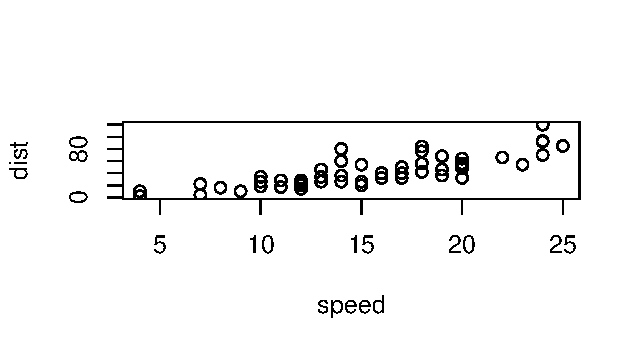
\includegraphics[width=\textwidth]{cars.pdf} 
  \end{center}

  \item Find the numerical value of $2\pi$, to $4$ decimal places.
  \begin{verbatim}
  round(2 * pi, 4)
    
  ## [1] 6.2832
  \end{verbatim}

  \item Show that $e^{i\pi}+1=0$.
  \begin{align*}
  e^{i\pi}+1&=\cos\pi+i\sin\pi+1\\
  &=-1+i\times0+1=0
  \end{align*}
  
\end{enumerate}

% A comment that won't appear in the output.

\end{document}
